\documentclass[12pt,a4paper]{article}
\usepackage[utf8]{inputenc}
\usepackage[english]{babel}
\usepackage{amsmath}
\usepackage{amsfonts}
\usepackage{amssymb}
\usepackage{graphicx}
\usepackage[left=2.5cm,right=2.5cm,top=2.5cm,bottom=2.5cm]{geometry}
\author{Silvano Garnerone}
\title{Topological data analysis of spotting-probes pointclouds}
\begin{document}
    
\maketitle

Given a point cloud derived from three-dimensional probes locations we want to analyze the shape of data, for the purpose of studying statistics of chromosomal shapes in a given cell population, comparing different chromosomes and identifying recurrent topological patterns.
Topological Data Analysis (TDA) is a set of method allowing us to quantify the shape of the data in a rigorous manner. 
\begin{figure}[hbtp]
\centering
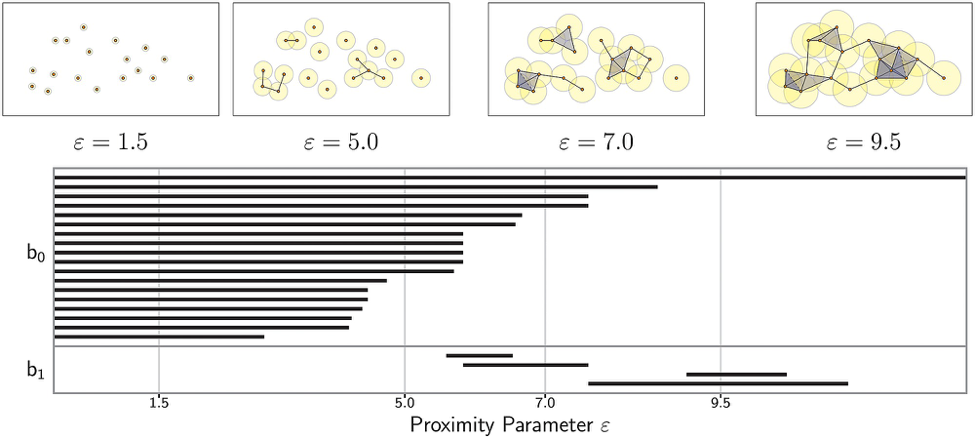
\includegraphics[scale=0.75]{PHbarcodeExample.png}
\caption{Example of persisten barcode.}
\label{fig:per_bc}
\end{figure}
As Fig.\ref{fig:per_bc} shows the idea is to expand spheres centered at each point, and while doing this to keep track of the number of connected components ($b_0$), holes ($b_1$) and voids ($b_2$, not shown in the figure) that emerge as a result of the expanding spheres radious ($\epsilon$). A summary of this information is provided by persistent diagrams (top part of Fig.\ref{fig:bc_pd}) and persistent barcodes (bottom part of Fig.\ref{fig:bc_pd}):
\begin{figure}[hbtp]
\centering
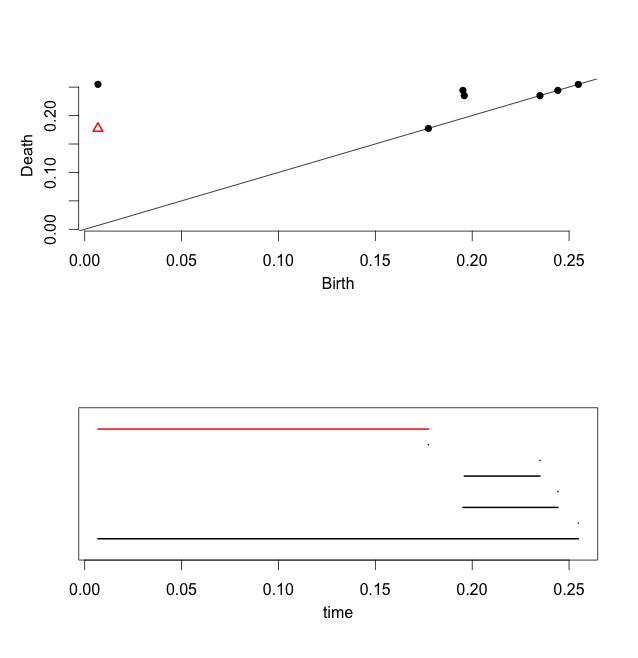
\includegraphics[scale=0.75]{rplot01.png}
\caption{Example of corresponding persistent diagram and persisten barcode, containing the same information.}
\label{fig:bc_pd}
\end{figure}
One can then compare different topological summaries using the bottleneck and the Wasserstein distances.

\section{Example with real data}
Let's consider the following dataset (iEG408\_003\_d0\_a594\/014\_006\_1.csv):
\begin{figure}[hbtp]
\centering
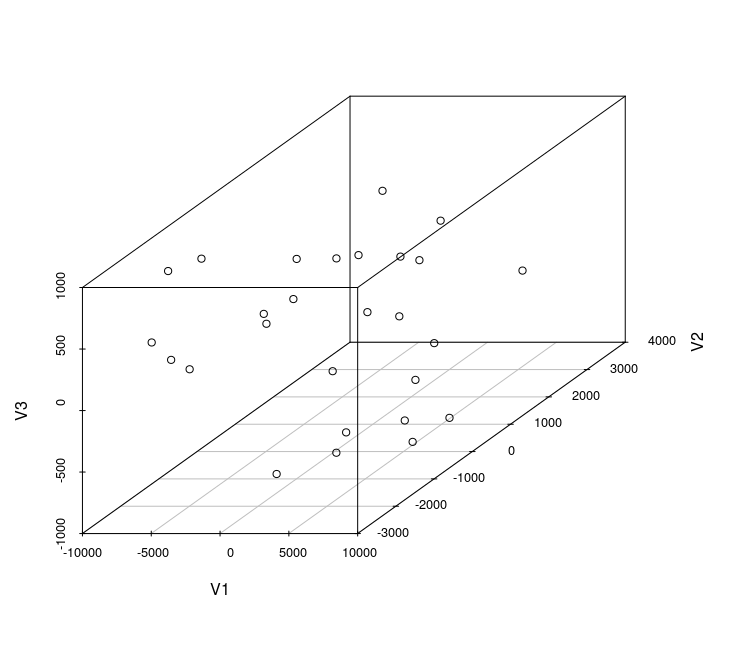
\includegraphics[scale=0.75]{a594_014_006_1.png}
\caption{Example of point cloud for chr20, first homologue.}
\label{pointcloud}
\end{figure}
applying TDA we get the following diagrams summarizing the start (birth) and end (death) of clusters (in black), loops (in red) and voids (in blue):
\begin{figure}[hbtp]
\centering
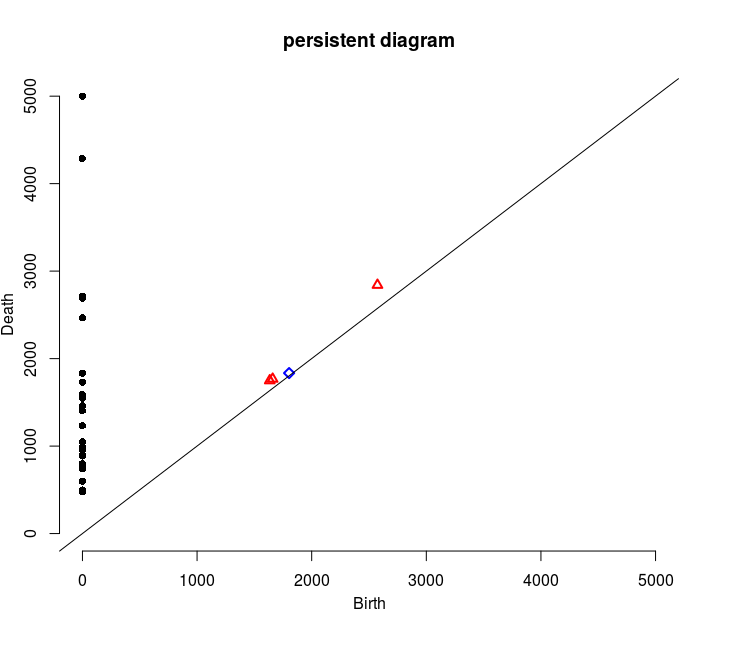
\includegraphics[scale=0.75]{p_dia.png}
\caption{Example of persistent diagram for chr20, first homologue.}
\end{figure}

\begin{figure}[hbtp]
\centering
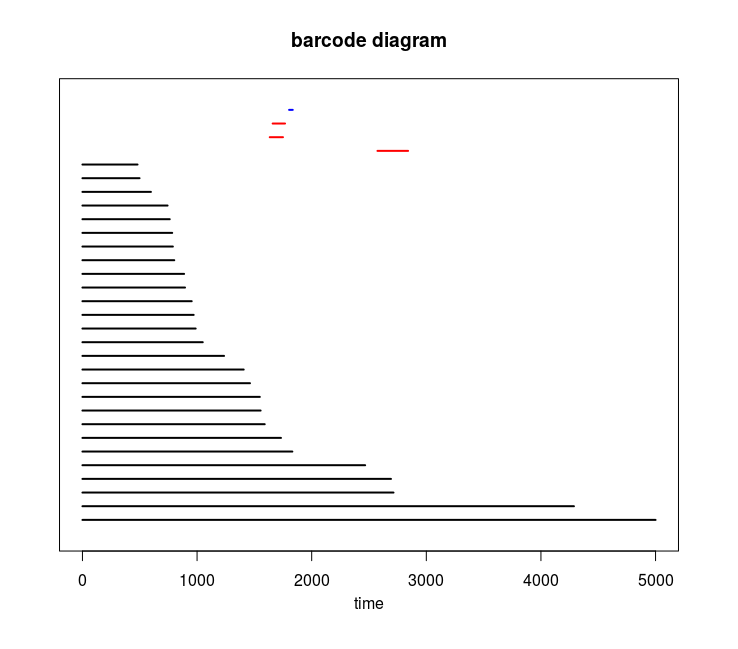
\includegraphics[scale=0.75]{bc_dia.png}
\caption{Example of barcode for chr20, first homologue.}
\end{figure}

Now let's consider a second dataset (iEG408\_003\_d0\_a594\/014\_006\_2.csv), the other homologue in the pair observed in the same nucleus. From this one we have the following plots:
\begin{figure}[hbtp]
\centering
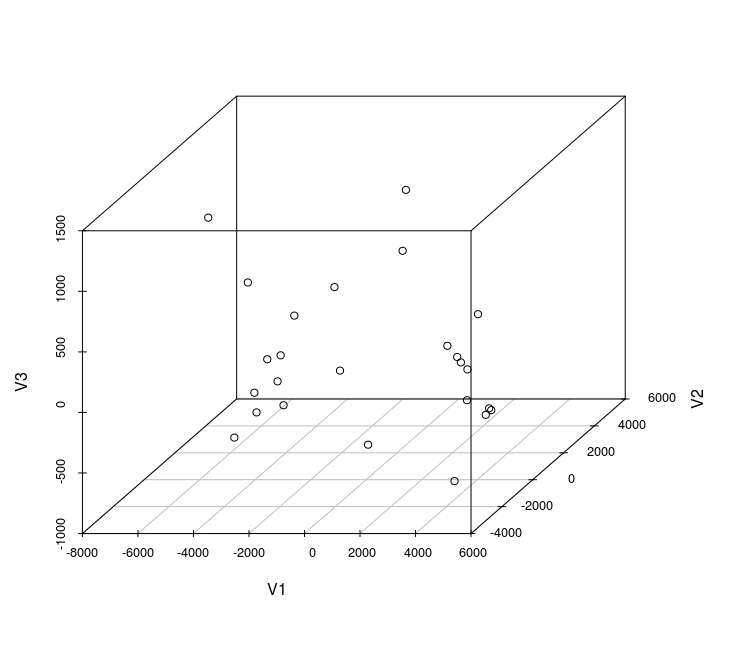
\includegraphics[scale=0.75]{a594_014_006_2.png}
\caption{Example of point cloud for chr20, second homologue.}
\end{figure}

\begin{figure}[hbtp]
\centering
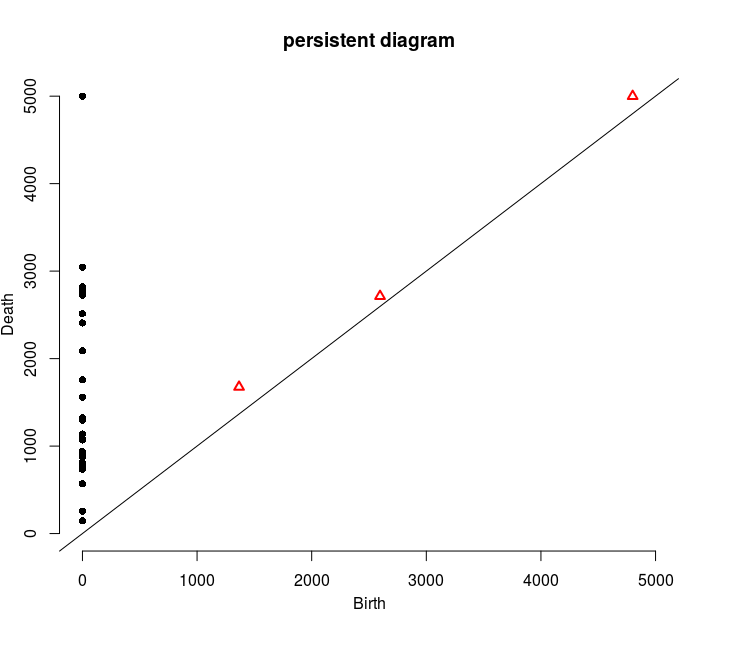
\includegraphics[scale=0.75]{p_dia_2.png}
\caption{Example of persistent diagram for chr20, second homologue.}
\end{figure}

\begin{figure}[hbtp]
\centering
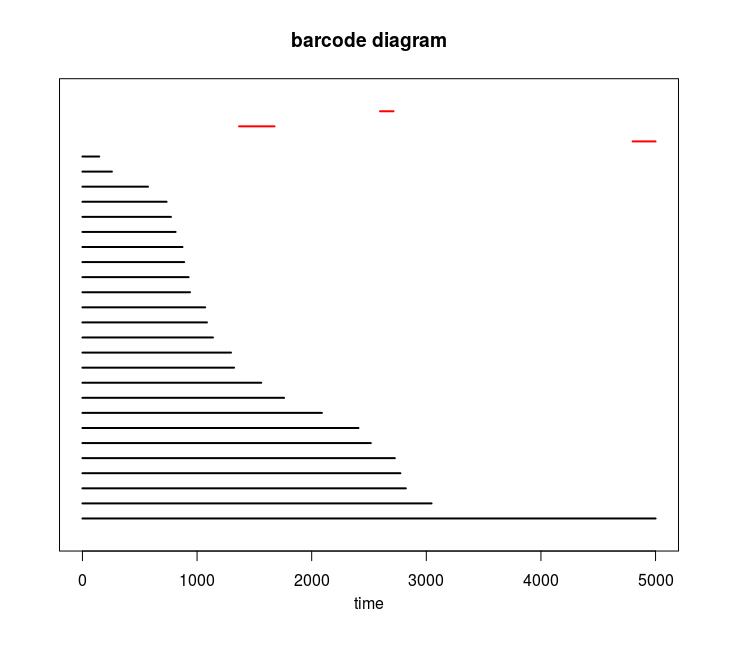
\includegraphics[scale=0.75]{bc_dia_2.png}
\caption{Example of barcode for chr20, second homologue.}
\end{figure}
Having a pair of point clouds it is also possible to quantify the similarity between their topological features, and quantify the fluctuations present in the topological summary of the point-clouds.

\section{Statistics of distances between topological summaries}
Given two point clouds, for each we evaluate the persistent diagram and then we take the p-Wassertein distance (with p=2) between the two diagrams, divided by the number of points in the larger cloud of the pair. The distance is a function D depending on chr\#1, chr\#2, and the dimension of the homological features (i.e. clusters, loops or voids). To start we consider the case where chr\#1=chr\#2=chromosome 1 (dataset IEG364-004 with 16 clouds with at least 20 points) and we plot the distribution of distances between all point clouds with at least 20 points (see Fig.\ref{fig:dist_0d_intra_chr1},\ref{fig:dist_1d_intra_chr1}). We then consider chromosome 20 (dataset iEG408-003-d0-a594 with 28 clouds with at least 20 points, 
see Fig.\ref{fig:dist_0d_intra_chr20},\ref{fig:dist_1d_intra_chr20}), and 
chromosome 2 (dataset iEG408-003-d0-cy5 with 69 clouds with at least 20 points, 
see Fig.\ref{fig:dist_0d_intra_chr2},\ref{fig:dist_1d_intra_chr2}).

\begin{figure}[hbtp]
\centering
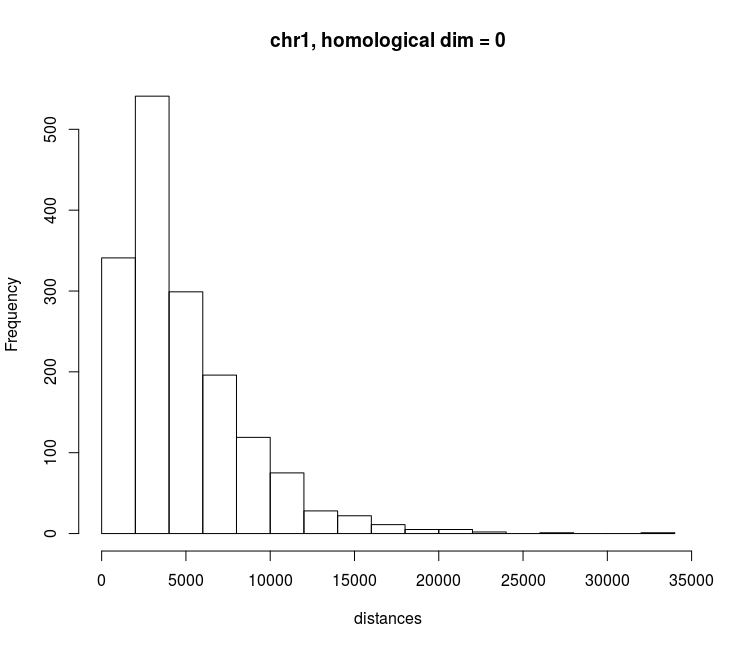
\includegraphics[scale=0.75]{2wd_chr1_dim0_16clouds.png}
\caption{Intra-chromosomal distances for all pair of point clouds, considering only the 0-th homological dimension.}
\label{fig:dist_0d_intra_chr1}
\end{figure}

\begin{figure}[hbtp]
\centering
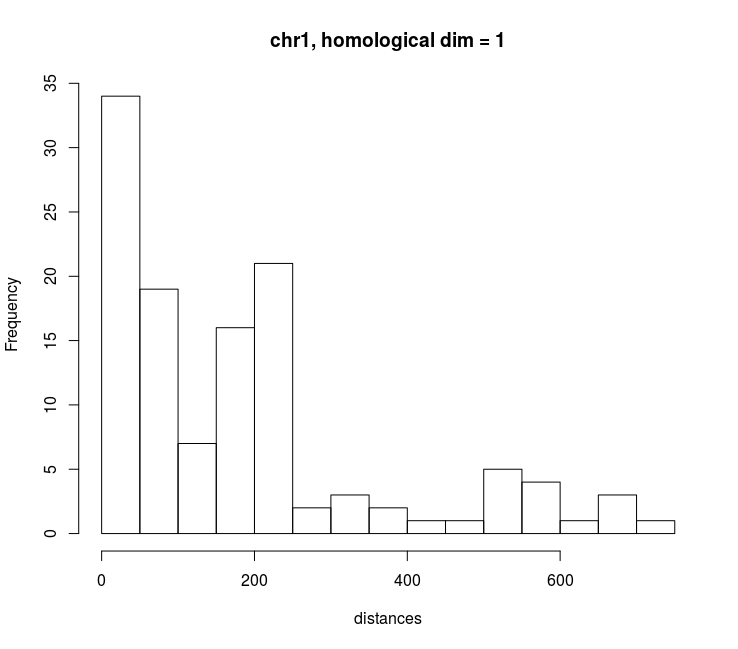
\includegraphics[scale=0.75]{2wd_chr1_dim1_16clouds.png}
\caption{Intra-chromosomal distances for all pair of point clouds, considering only the 1-st homological dimension.}
\label{fig:dist_1d_intra_chr1}
\end{figure}

\begin{figure}[hbtp]
\centering
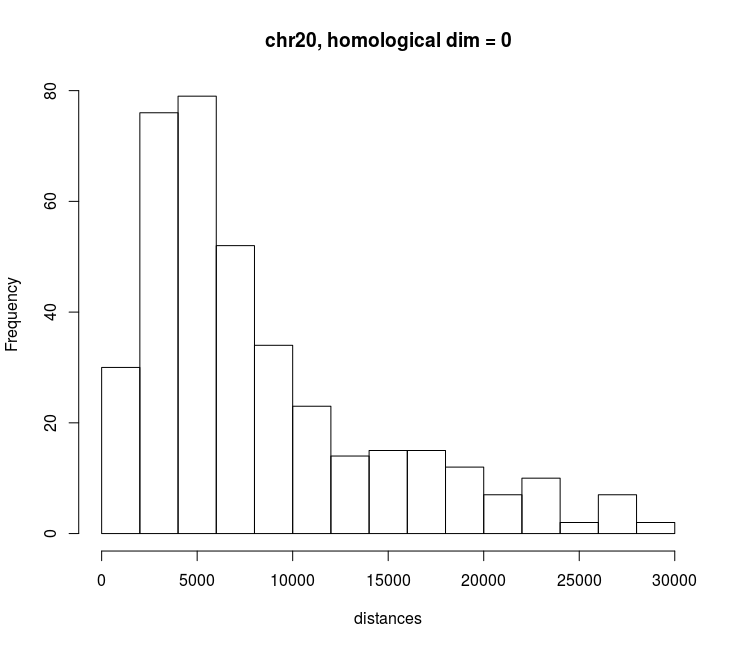
\includegraphics[scale=0.75]{2wd_chr20_dim0_28clouds.png}
\caption{Intra-chomosomal distances in the 0-th homological dimension space.}
\label{fig:dist_0d_intra_chr20}
\end{figure}

\begin{figure}[hbtp]
\centering
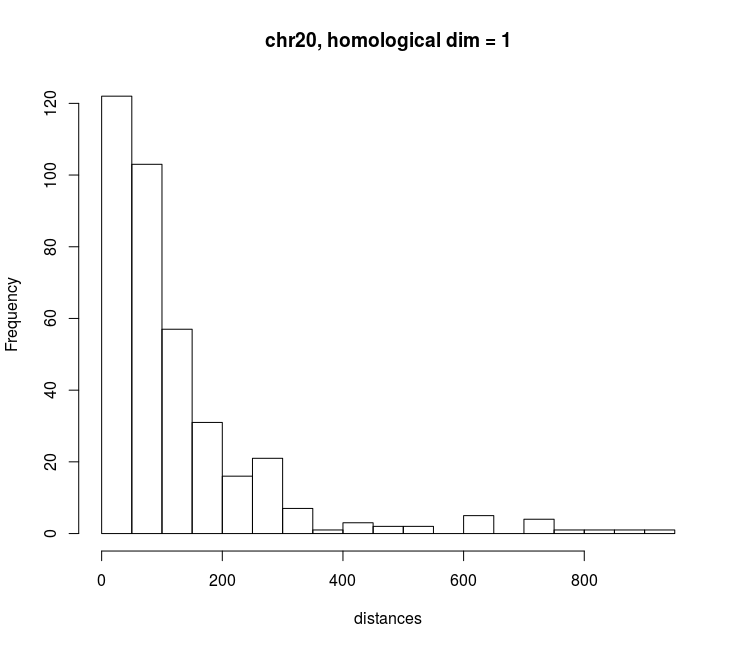
\includegraphics[scale=0.75]{2wd_chr20_dim1_28clouds.png}
\caption{Intra-chomosomal distances in the 1-st homological dimension space.}
\label{fig:dist_1d_intra_chr20}
\end{figure}

\begin{figure}[hbtp]
\centering
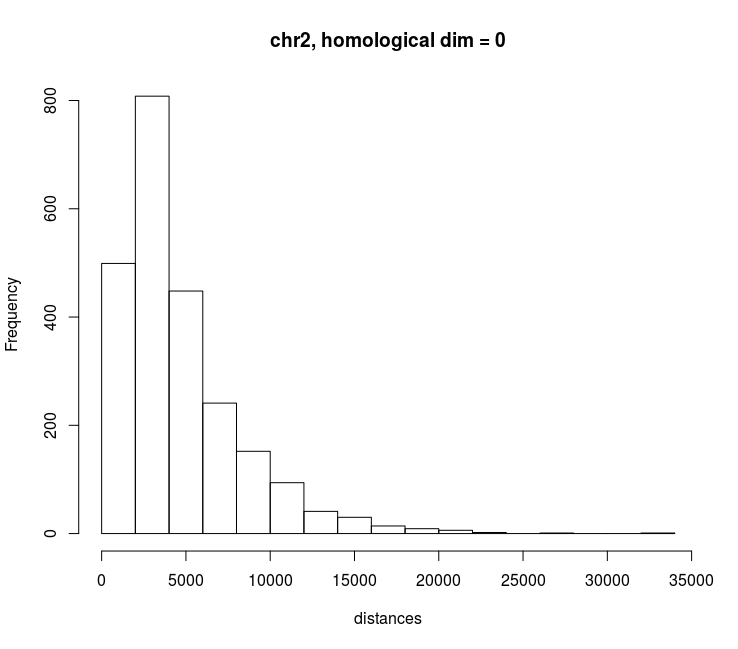
\includegraphics[scale=0.75]{2wd_chr2_dim0_69clouds.png}
\caption{Intra-chomosomal distances in the 0-th homological dimension space.}
\label{fig:dist_0d_intra_chr2}
\end{figure}
\begin{figure}[hbtp]
\centering
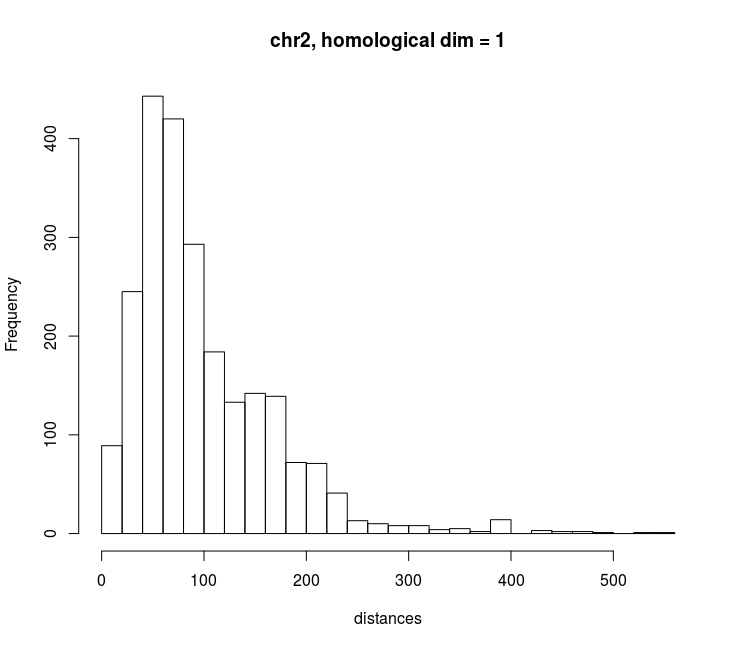
\includegraphics[scale=0.75]{2wd_chr2_dim1_69clouds.png}
\caption{Intra-chomosomal distances in the 1-st homological dimension space.}
\label{fig:dist_1d_intra_chr2}
\end{figure}

Fig.\ref{fig:vio_d0_intra} shows a violin plot summarizing the statistics for dim = 0 (clusters), 
while Fig.\ref{fig:vio_d1_intra} shows the same for 1-dim features.
\begin{figure}[hbtp]
\centering
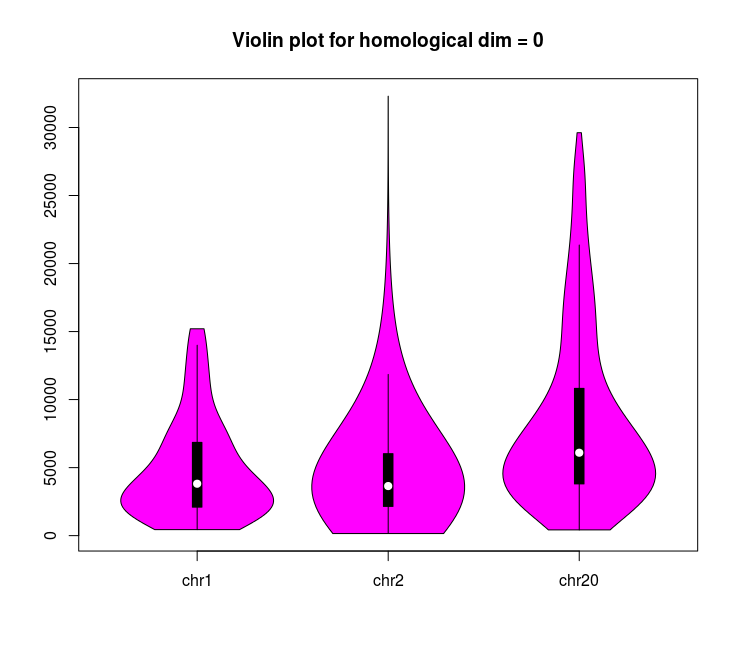
\includegraphics[scale=0.75]{violin_plot_dim0.png}
\caption{Violin plot of intra-chromosomal 0-dim distances.}
\label{fig:vio_d0_intra}
\end{figure}

\begin{figure}[hbtp]
\centering
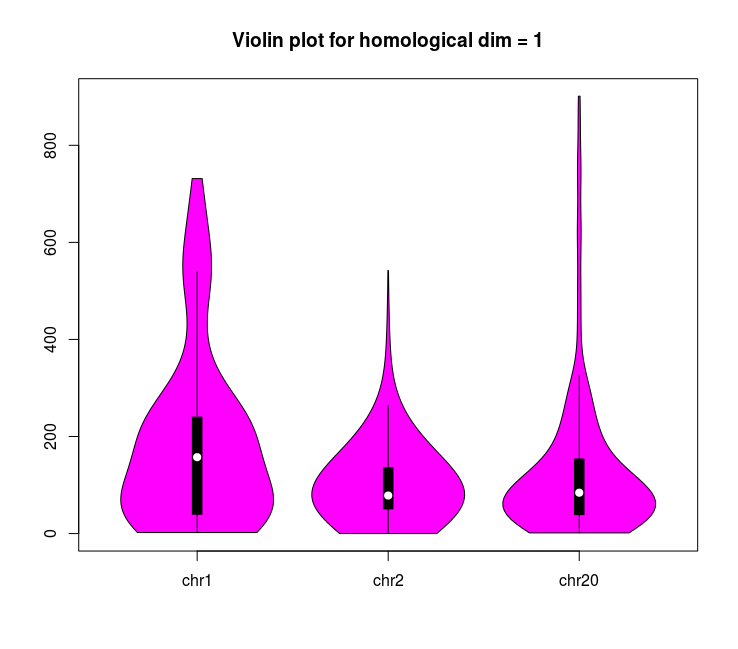
\includegraphics[scale=0.75]{violin_plot_dim1.png}
\caption{Violin plot of intra-chromosomal 1-dim distances.}
\label{fig:vio_d1_intra}
\end{figure}

Bringing all the different violin plots together we can compare intra- and inter-chromosomal topological fluctuations (see Fig.\ref{fig:vio_d0_intra},\ref{fig:vio_d1_intra},\ref{fig:vio_d0_inter},\ref{fig:vio_d1_inter}).
\begin{figure}[hbtp]
\centering
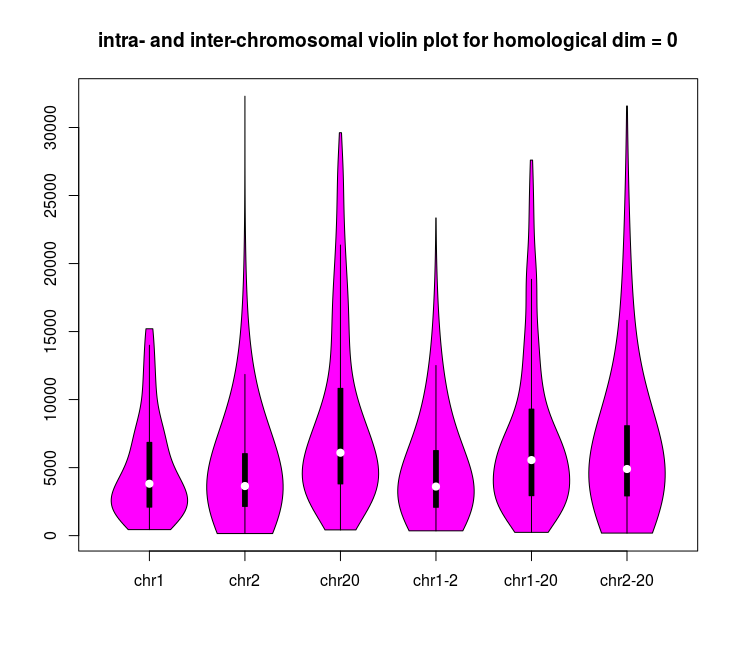
\includegraphics[scale=0.75]{fluct_dim0.png}
\caption{Violin plot of intra and inter-chromosomal homological distances in dim 0.}
\label{fig:vio_d0_inter}
\end{figure}
\begin{figure}[hbtp]
\centering
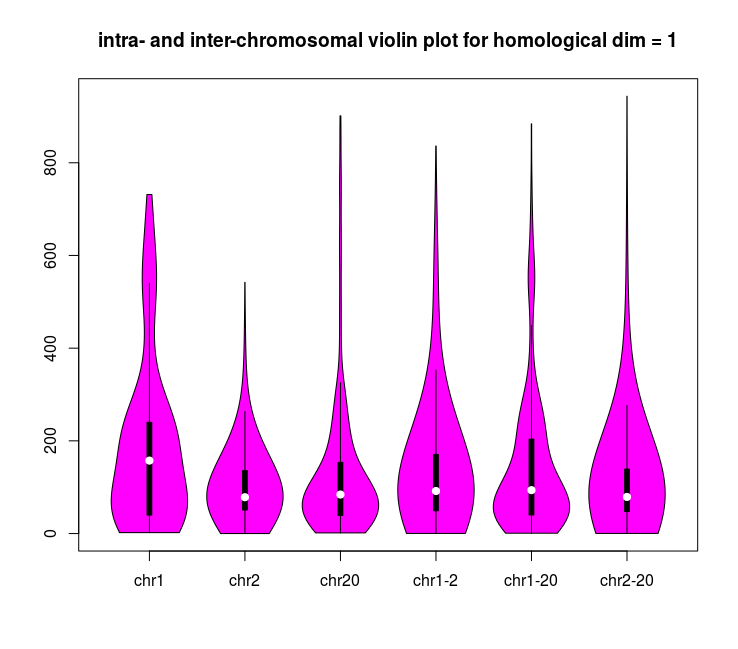
\includegraphics[scale=0.75]{fluct_dim1.png}
\caption{Violin plot of intra and inter-chromosomal homological distances in dim 1.}
\label{fig:vio_d1_inter}
\end{figure}

\section{Silhouettes}
Persistence silhouettes are real valued functions summarizing the information contained in a persistence diagram [REF]. 
Consider first the triangle function associated to a persistence diagram with N points, each defined by the pair (b,d) of birth and death coordinates:
\begin{equation}
\Lambda_p(t)=\left\{
\begin{array}{cc}
t-b & t \in [b,\frac{b+d}{2}] \\ 
d-t & t \in (\frac{b+d}{2},d] \\ 
0 & otherwise
\end{array}\right., 
\end{equation}
for every $0<p<\infty$ we define the power-weighted silhouette
\begin{equation}
\phi^{(p)}(t) = \frac{\sum_{j=1}^N \vert d_j-b_j \vert^p \Lambda_j(t)}{\sum_{j=1}^N \vert d_j - b_j\vert^p}.
\end{equation}
For statistical purposes, silhouettes are more convenient than persistent diagrams to deal with, since for example it is 
possible to unambiguously define the average of a collection of them. Fig\ref{fig:meanSil_chr1_dim0} to \ref{fig:meanSil_chr20_dim1} show the 
average, over different point clouds, and the 95\% confidence interval 
(obtained with a multiplier bootstrap method [REF]) of silhouettes in dim 0 and dim 1; these summaries can be used to classify and compare different chromosomes.

\begin{figure}[hbtp]
\centering
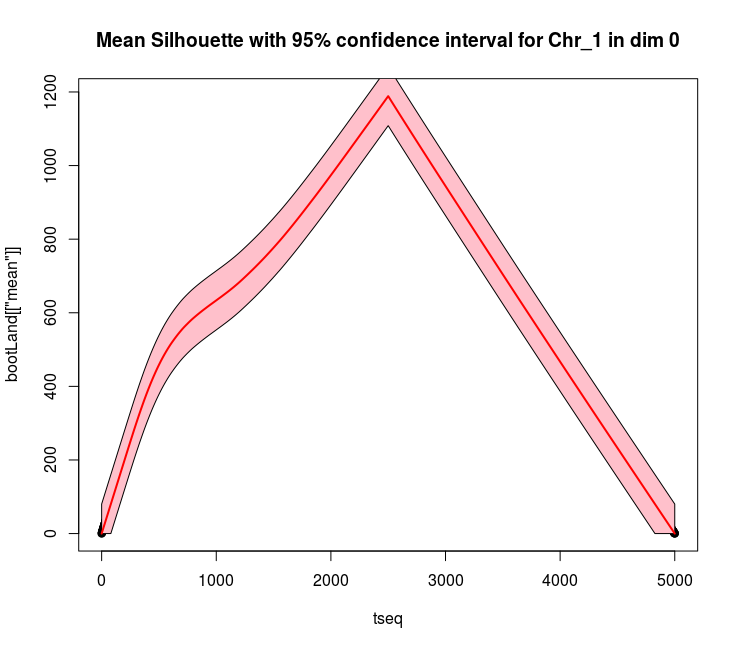
\includegraphics[scale=0.75]{meanSil_chr1_dim0.png}
\caption{Mean silhouette for chr 1, homological dimension 0.}
\label{fig:meanSil_chr1_dim0}
\end{figure}

\begin{figure}[hbtp]
\centering
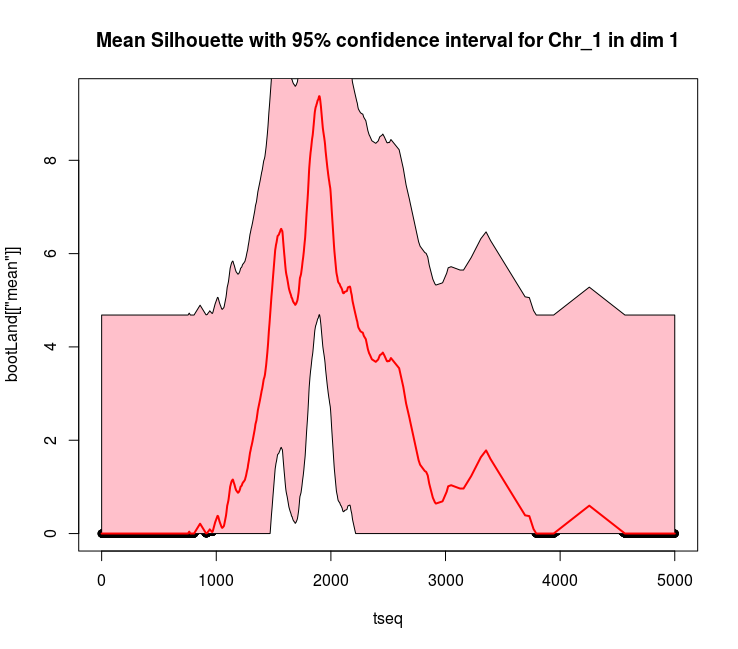
\includegraphics[scale=0.75]{meanSil_chr1_dim1.png}
\caption{Mean silhouette chr 1, homological dimension 1.}
\label{fig:meanSil_chr1_dim1}
\end{figure}

\begin{figure}[hbtp]
\centering
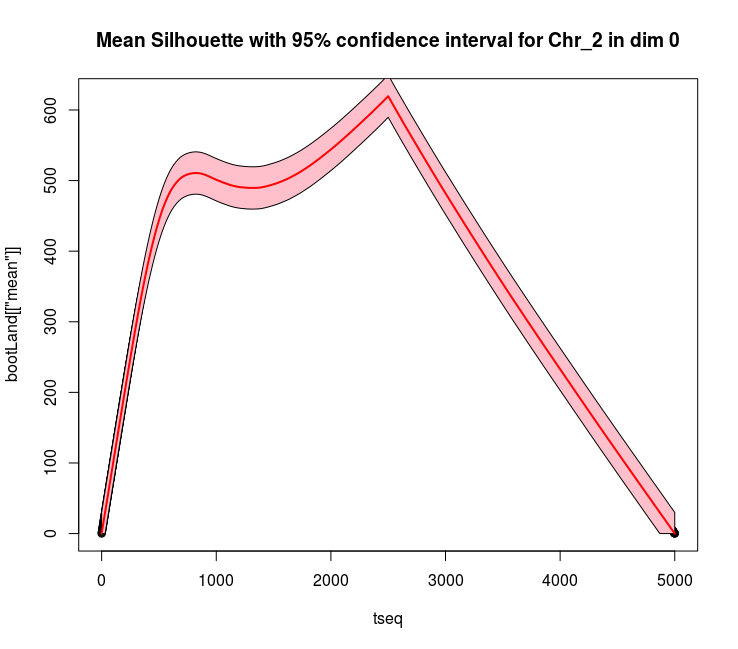
\includegraphics[scale=0.75]{meanSil_chr2_dim0.png}
\caption{Mean silhouette for chr 2, homological dimension 0.}
\label{fig:meanSil_chr2_dim0}
\end{figure}

\begin{figure}[hbtp]
\centering
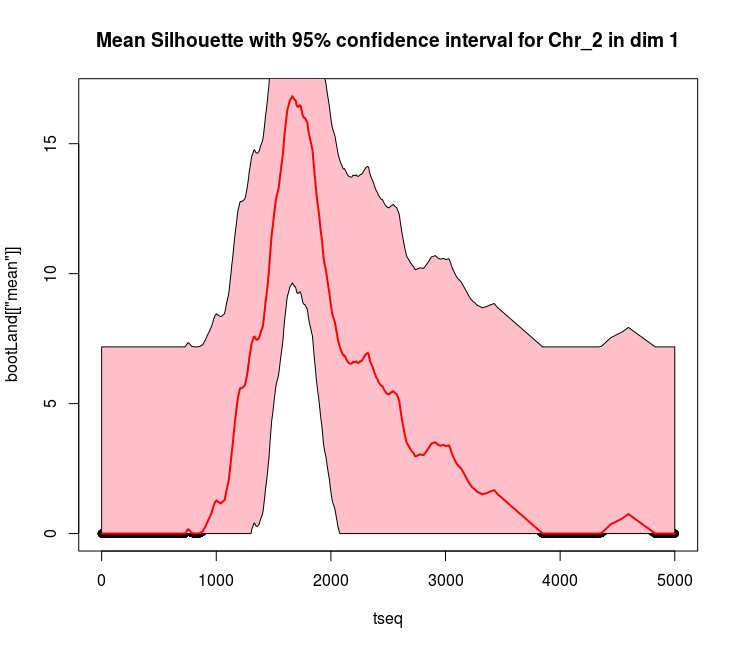
\includegraphics[scale=0.75]{meanSil_chr2_dim1.png}
\caption{Mean silhouette chr 2, homological dimension 1.}
\label{fig:meanSil_chr2_dim1}
\end{figure}

\begin{figure}[hbtp]
\centering
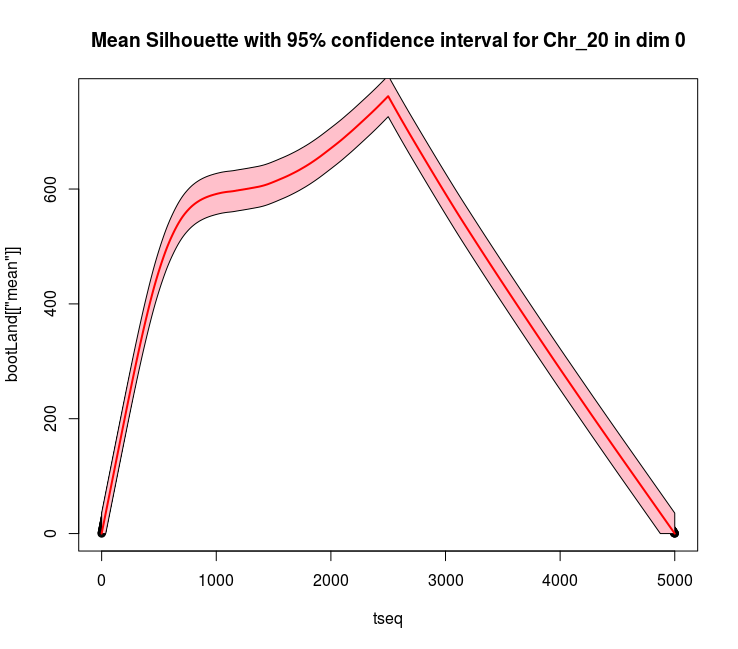
\includegraphics[scale=0.75]{meanSil_chr20_dim0.png}
\caption{Mean silhouette for chr 20, homological dimension 0.}
\label{fig:meanSil_chr20_dim0}
\end{figure}

\begin{figure}[hbtp]
\centering
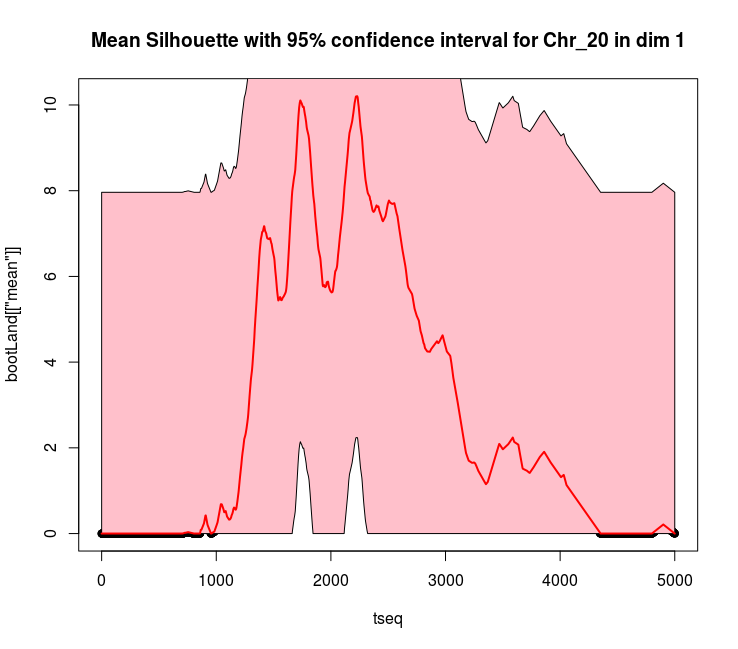
\includegraphics[scale=0.75]{meanSil_chr20_dim1.png}
\caption{Mean silhouette chr 20, homological dimension 1.}
\label{fig:meanSil_chr20_dim1}
\end{figure}



\end{document}
